\chapter{Introduction}

\section{Who was Kowalevski?}
\begin{wrapfigure}{i}{0.25\textwidth}
    \centering
    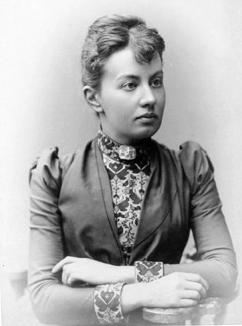
\includegraphics[width=0.25\textwidth]{kovalevskaya_8}
\end{wrapfigure}

Sofya Vasilyevna Kovalevskaya (1850-1891) was a Russian mathematician. For various reasons, including the theorem central to this discussion, she remains one of the most prominent female figures in the history of this discipline.

First of all, it is important to note that, from this point forward, we will often refer to her by the name she used to sign her publications, i.e., Kowalevski.

In order to leave Russia, she entered into a marriage of convenience, marrying a man with whom she had no real emotional relationship for several years and from whom she was often geographically distant.
This allowed her to continue her studies in Germany, where she met Karl Weierstrass, one of the most influential mathematicians of his time.
After their initial meeting in the professor's study, their relationship continued to develop due to Kowalevski's evident mathematical talents, which Weierstrass could not help but nurture. He continued to give her private lessons and eventually supervised her research work.

Regarding Kowalevski's political views, we can say with historical certainty that she was close to feminist movements and socialist and radical ideas, which can be traced back to her family background and the influences she encountered during her life in modern-day European states. It is certainly noteworthy that she received several copies of radical magazines from her sister Anna, which discussed the so-called Russian nihilism\footnote{science, not religion or superstition, was considered by Russian nihilists to be the most effective means of helping the population lead better lives and thus represented truth and progress.}.

However, we want to focus on her contribution to mathematics rather than her political, social, and philosophical ideas. With the help of what we might call her mentor, Kowalevski made several important discoveries. After years of collaboration, she published three doctoral theses in a single year: 1874. This is remarkable not only for the sheer volume but also because she became the first woman to earn a PhD, thanks in part to the support of Weierstrass, as revealed in a letter he wrote to his colleague Fuchs at the University of Berlin regarding the approval of Kowalevski's theses. 

Moreover, her publications turned out to be milestones in mathematics. In particular, the topics covered are:
\begin{itemize}
\item Partial differential equations (PDE), Cauchy-Kowalevski theorem
\item Mechanics, Kowalevski top
\item Elliptic integrals
\end{itemize}

After the success, which was naturally followed by some awards, she returned to Russia for a period; however, this proved to be futile for the continuation of her academic career. Later, when the husband to whom she owed the opportunity to study in Germany passed away, she moved to Sweden, where she achieved another first: she became the world's first female professor of mathematics, obtaining a position at Stockholm University.
Unfortunately, her life was cut short at the age of 41 by pneumonia, which, according to sources, prevented her from pursuing her great passion for literary production.
Despite not being able to express herself in this field as she would have liked, there are numerous artistic representations of her, both in literature and cinema.

Here are some of the major cinematic works:
\begin{itemize}
\emergencystretch 3em
\item \textit{Sofya Kowalevski}(1985, Lenfilm, 3 episodes, 218 minutes), Ayan Gasanovna Shakhmaliyeva (1932-1999, originally from Azerbaijan).

\item \textit{A Hill on the Dark Side of the Moon} (Swedish: \textit{Berget på månens baksida})(1983), Lennart Hjulström (1938-2022)
\end{itemize}

Here are some of the major literary works:
\begin{itemize}

\item a biography: \textit{Sonja Kovalevsky. What I Lived With Her and What She Told Me About Herself} (1892, Ed. Albert Bonniers, Stockholm), Anne Charlotte Leffler (a close friend of Kowalevski, sister of mathematician Gösta Mittag-Leffler and wife of the Italian algebraist Pasquale del Pezzo)

\item an autobiography: \textit{A Russian Childhood} (1978, Springer New York, NY), Sofya Kovalevskaya, translated and edited by Beatrice Stillman

\item a biography: \textit{Little Sparrow: A Portrait of Sophia Kovalevsky} (1983, Ohio University Press, Athens, Ohio), Don H. Kennedy

\item a biographical novel: \textit{Beyond the Limit: The Dream of Sofya Kovalevskaya} (2002, Tom Doherty Associates, LLC), Joan Spicci (mathematician and educator)

\item a biographical short story: \textit{Too Much Happiness}\footnote{this story recounts the last days of Kowalevski's life enriched with reminiscences of the past that Munro acquired from letters, diaries, and writings (documents she accessed through Don H. Kennedy's wife, a distant relative of Kowalevski)} (2009, Harper's Magazine), Alice Munro (1931-2024, Nobel Prize in Literature)

\end{itemize}

\section{The Cauchy-Kowalevski Theorem}\label{introck}

Having introduced the historical figure, we can now take the first step toward exploring one of Kowalevski's major works: the Cauchy-Kowalevski theorem, which we will abbreviate as CKT from now on.

\emergencystretch 3em
First, let us quickly describe the scientific context of the time concerning PDEs.

The father of the research carried out in the 19th century was Augustin-Louis Cauchy, a mathematician likely well-known to the reader. During those years, particularly between 1835 and 1842, Cauchy was developing the theory of holomorphic functions, already initiated by other major figures like Euler, Laplace, and Fourier.

Cauchy had the intuition to apply these results to differential equations.

It is important to grasp, with the mindset of that era, that classical theory and power series were promising tools, primarily for their simplicity and elegance, but also for the approximation potential of a simple truncation of a series.

Cauchy's attempt to apply the tools from his research to differential equations was successful, but only partially, for one simple reason: he was unable to go beyond the study of ordinary differential equations (ODEs) and linear PDEs.

The breakthrough came thanks to Kowalevski and Weierstrass. The latter was very optimistic about the results he thought could be achieved, perhaps even more so than Cauchy: he conjectured that it would be possible to define analytic functions via differential equations, using formal power series derived from the equations' expressions.
For this reason, he encouraged Kowalevski, with her talent, to delve deeper into this subject.

However, it would be wrong to think that Kowalevski's guides were only Cauchy and Weierstrass: other mathematicians also worked on these topics, including Briot, Bouquet, and Fuchs, who further developed the concepts of singularities, and Jacobi, who was the first to define the normal form of an equation\footnote{this concept, in particular, would prove crucial in Kowalevski's research}.

Building on these foundations, Kowalevski's key idea can be summarized as follows:
\begin{enumerate}
\item perform a variable change that allows a nonlinear equation to be written in normal form (see chapters \ref{tools} and \ref{invariant} for the meaning of this term), maintaining regularity assumptions on the data, and address the existence of a solution for this system;
\item transform any equation in normal form into a particular quasi-linear system;
\item apply to this system the majorant method already used by Cauchy for his discoveries on ODEs and linear PDEs.
\end{enumerate}

As often happens in mathematics, the proof was later simplified by E. Goursat in his mathematics textbook from around 1900. Moreover, over time, more abstract and general statements and proofs were proposed, thanks to the work of Ovsyannikov, Treves, and Nirenberg.

It should be noted that, during the same period, Darboux also achieved results very similar to Kowalevski, but with less generality.

\newpage

In light of what has been said so far, we pose some crucial questions, to which we seek the most comprehensive answers possible, and which will guide our discussion:
\begin{itemize}
\item is it possible for a system of PDEs with Cauchy data to have an analytic solution?
\end{itemize}
If so,
\begin{itemize}
\item under what assumptions?
\item is the solution unique?
\item does the solution depend continuously on the data?
\item what are the consequences and applications of the results obtained?
\end{itemize}
